\section{The K-mer Representation Quality} \label{sec:K_mer_Representation}

Investigation on the anomalies resulted in two persistent clustering errors \autoref{fig:PCA_Cluster_Knee_4} \textbf{\textsf{B}} and \textbf{\textsf{D}}. To evaluate if the method is suitable for the clustering of \gls{IAV} possible error sources are discussed.

% \begin{figure}[!hbt]
%     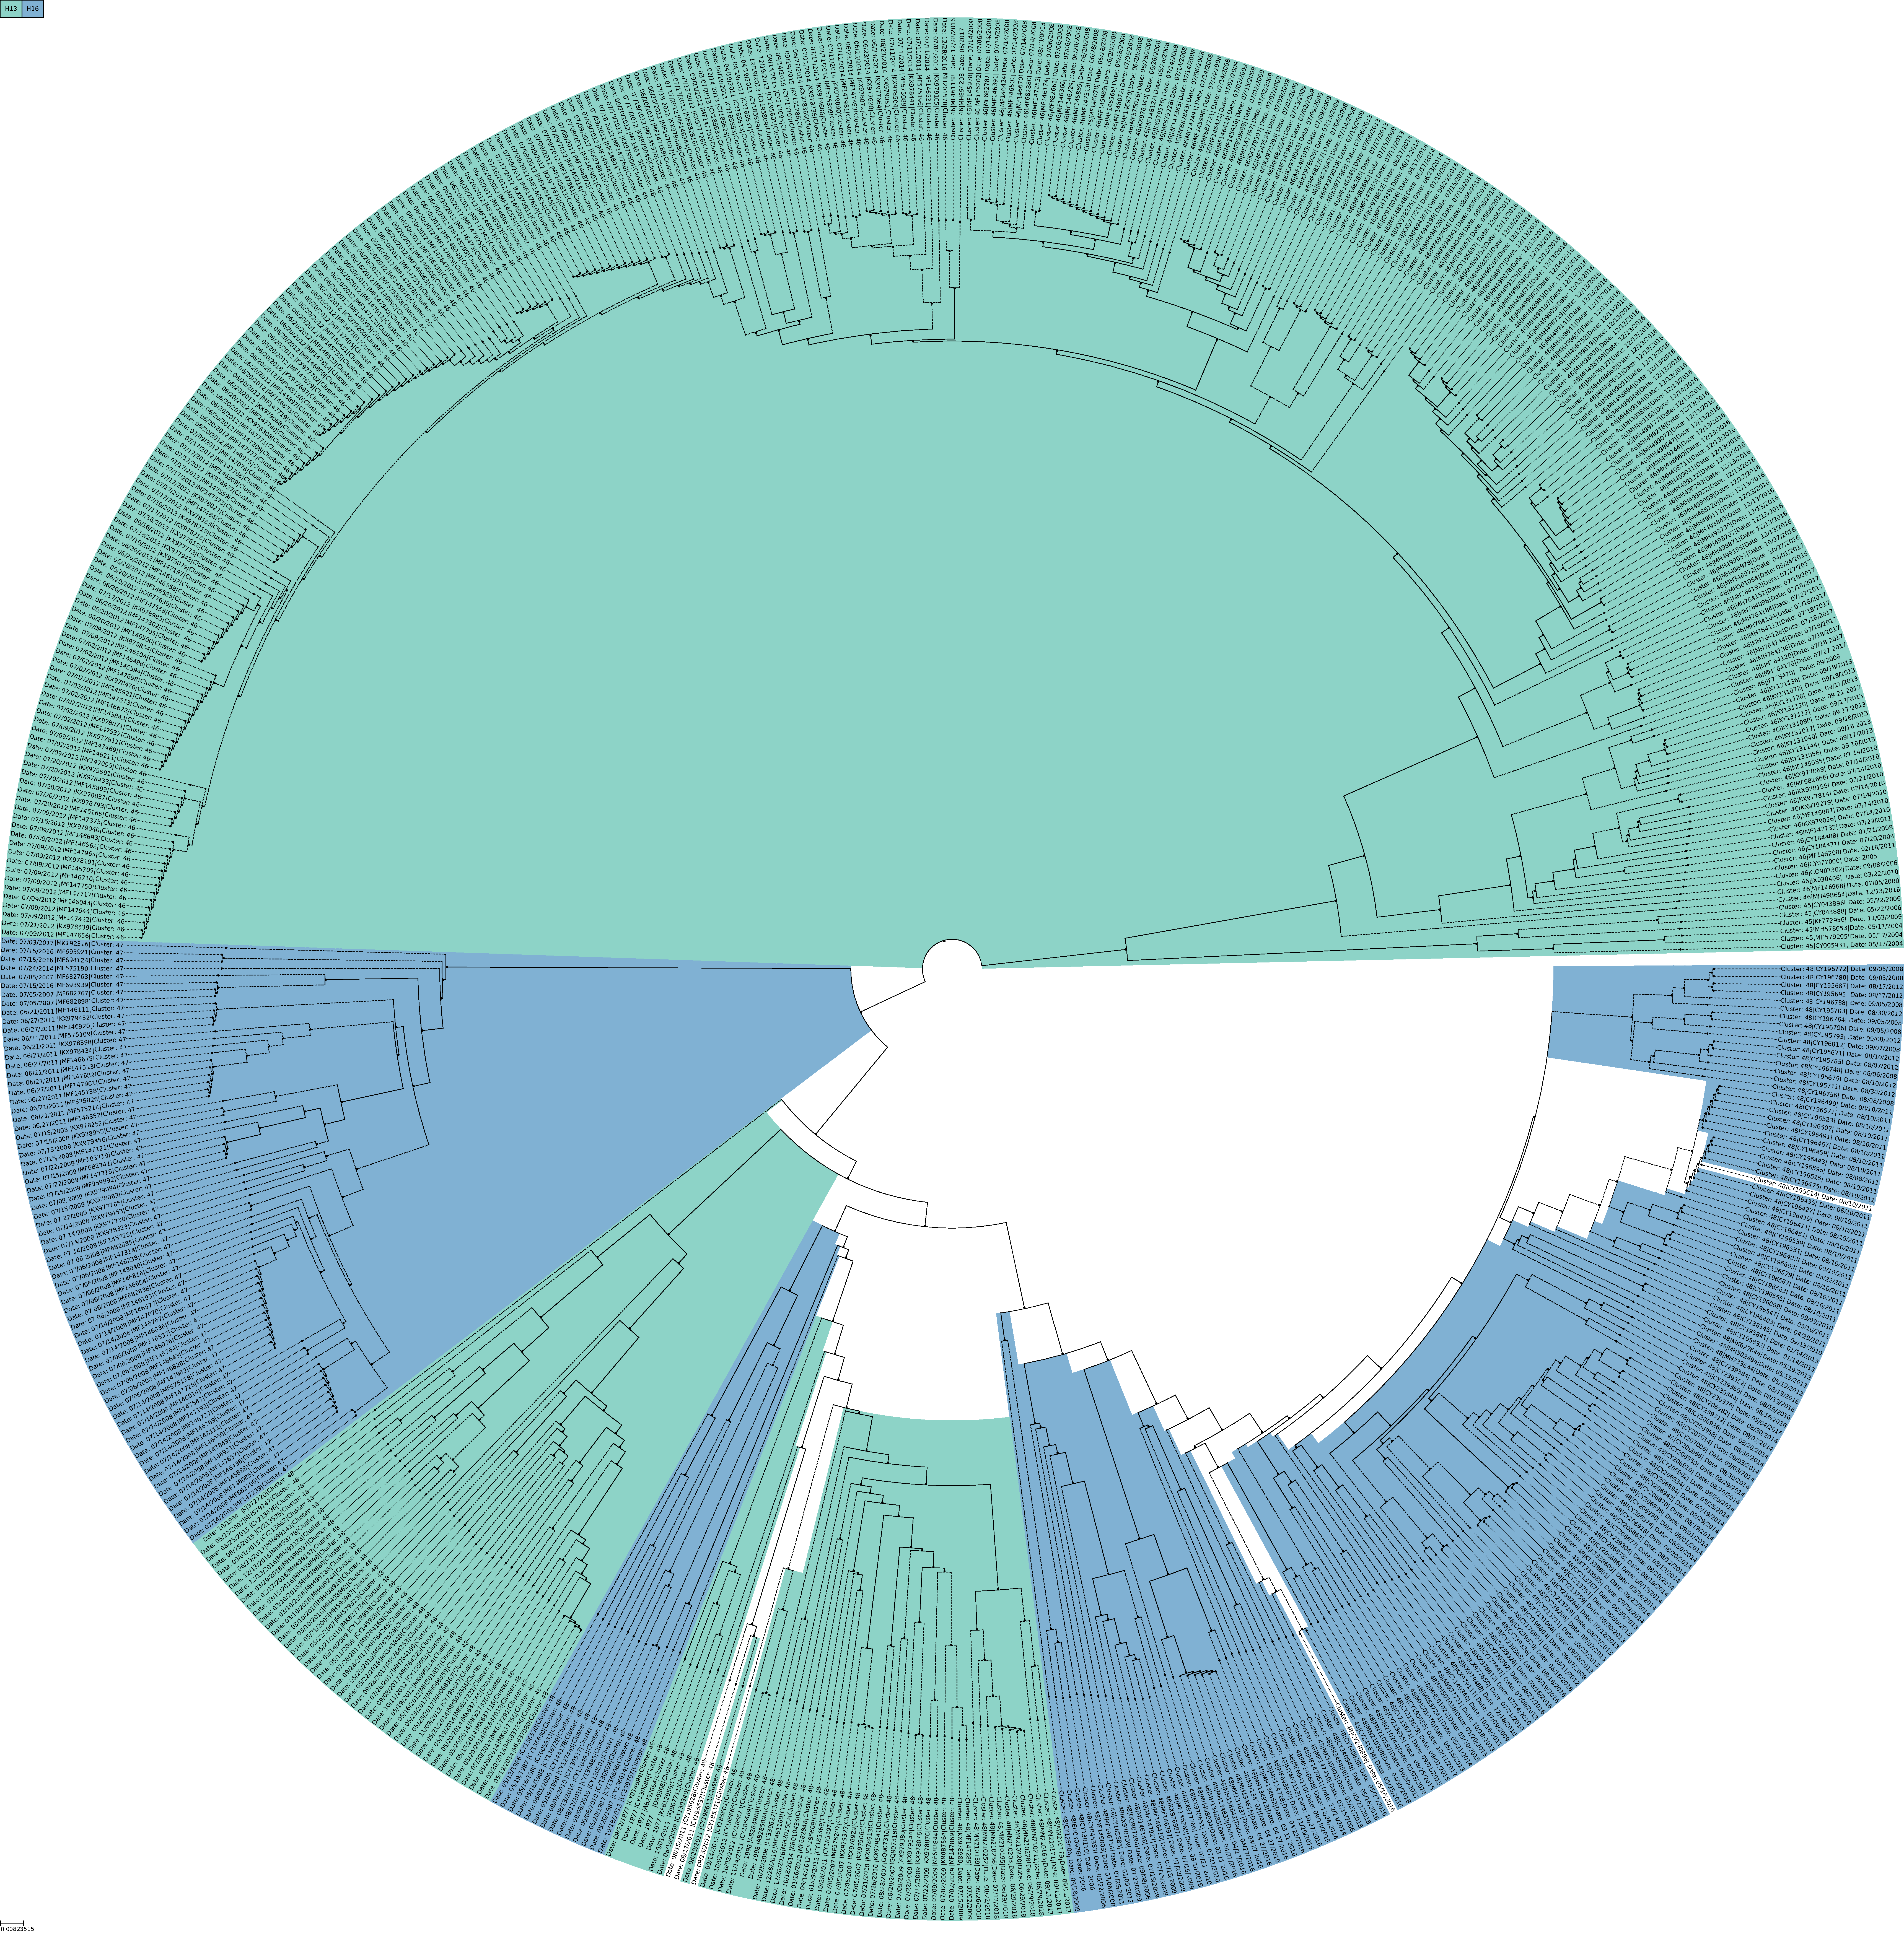
\includegraphics[width=\dimexpr\textwidth-2\fboxsep-2\fboxrule,fbox]{PCA/Clustertree_Segment_4_H_Knee_Zoom.pdf}
%     \caption[H13/H16 Simple Clustering Example with \Acrshort{PCA}]{\textbf{H13/H16 Simple Clustering Example with \Acrshort{PCA}.} .}
%     \label{fig:PCA_Clusteree_Knee_Zoom}
% \end{figure}

% \begin{figure}[!hbt]
%     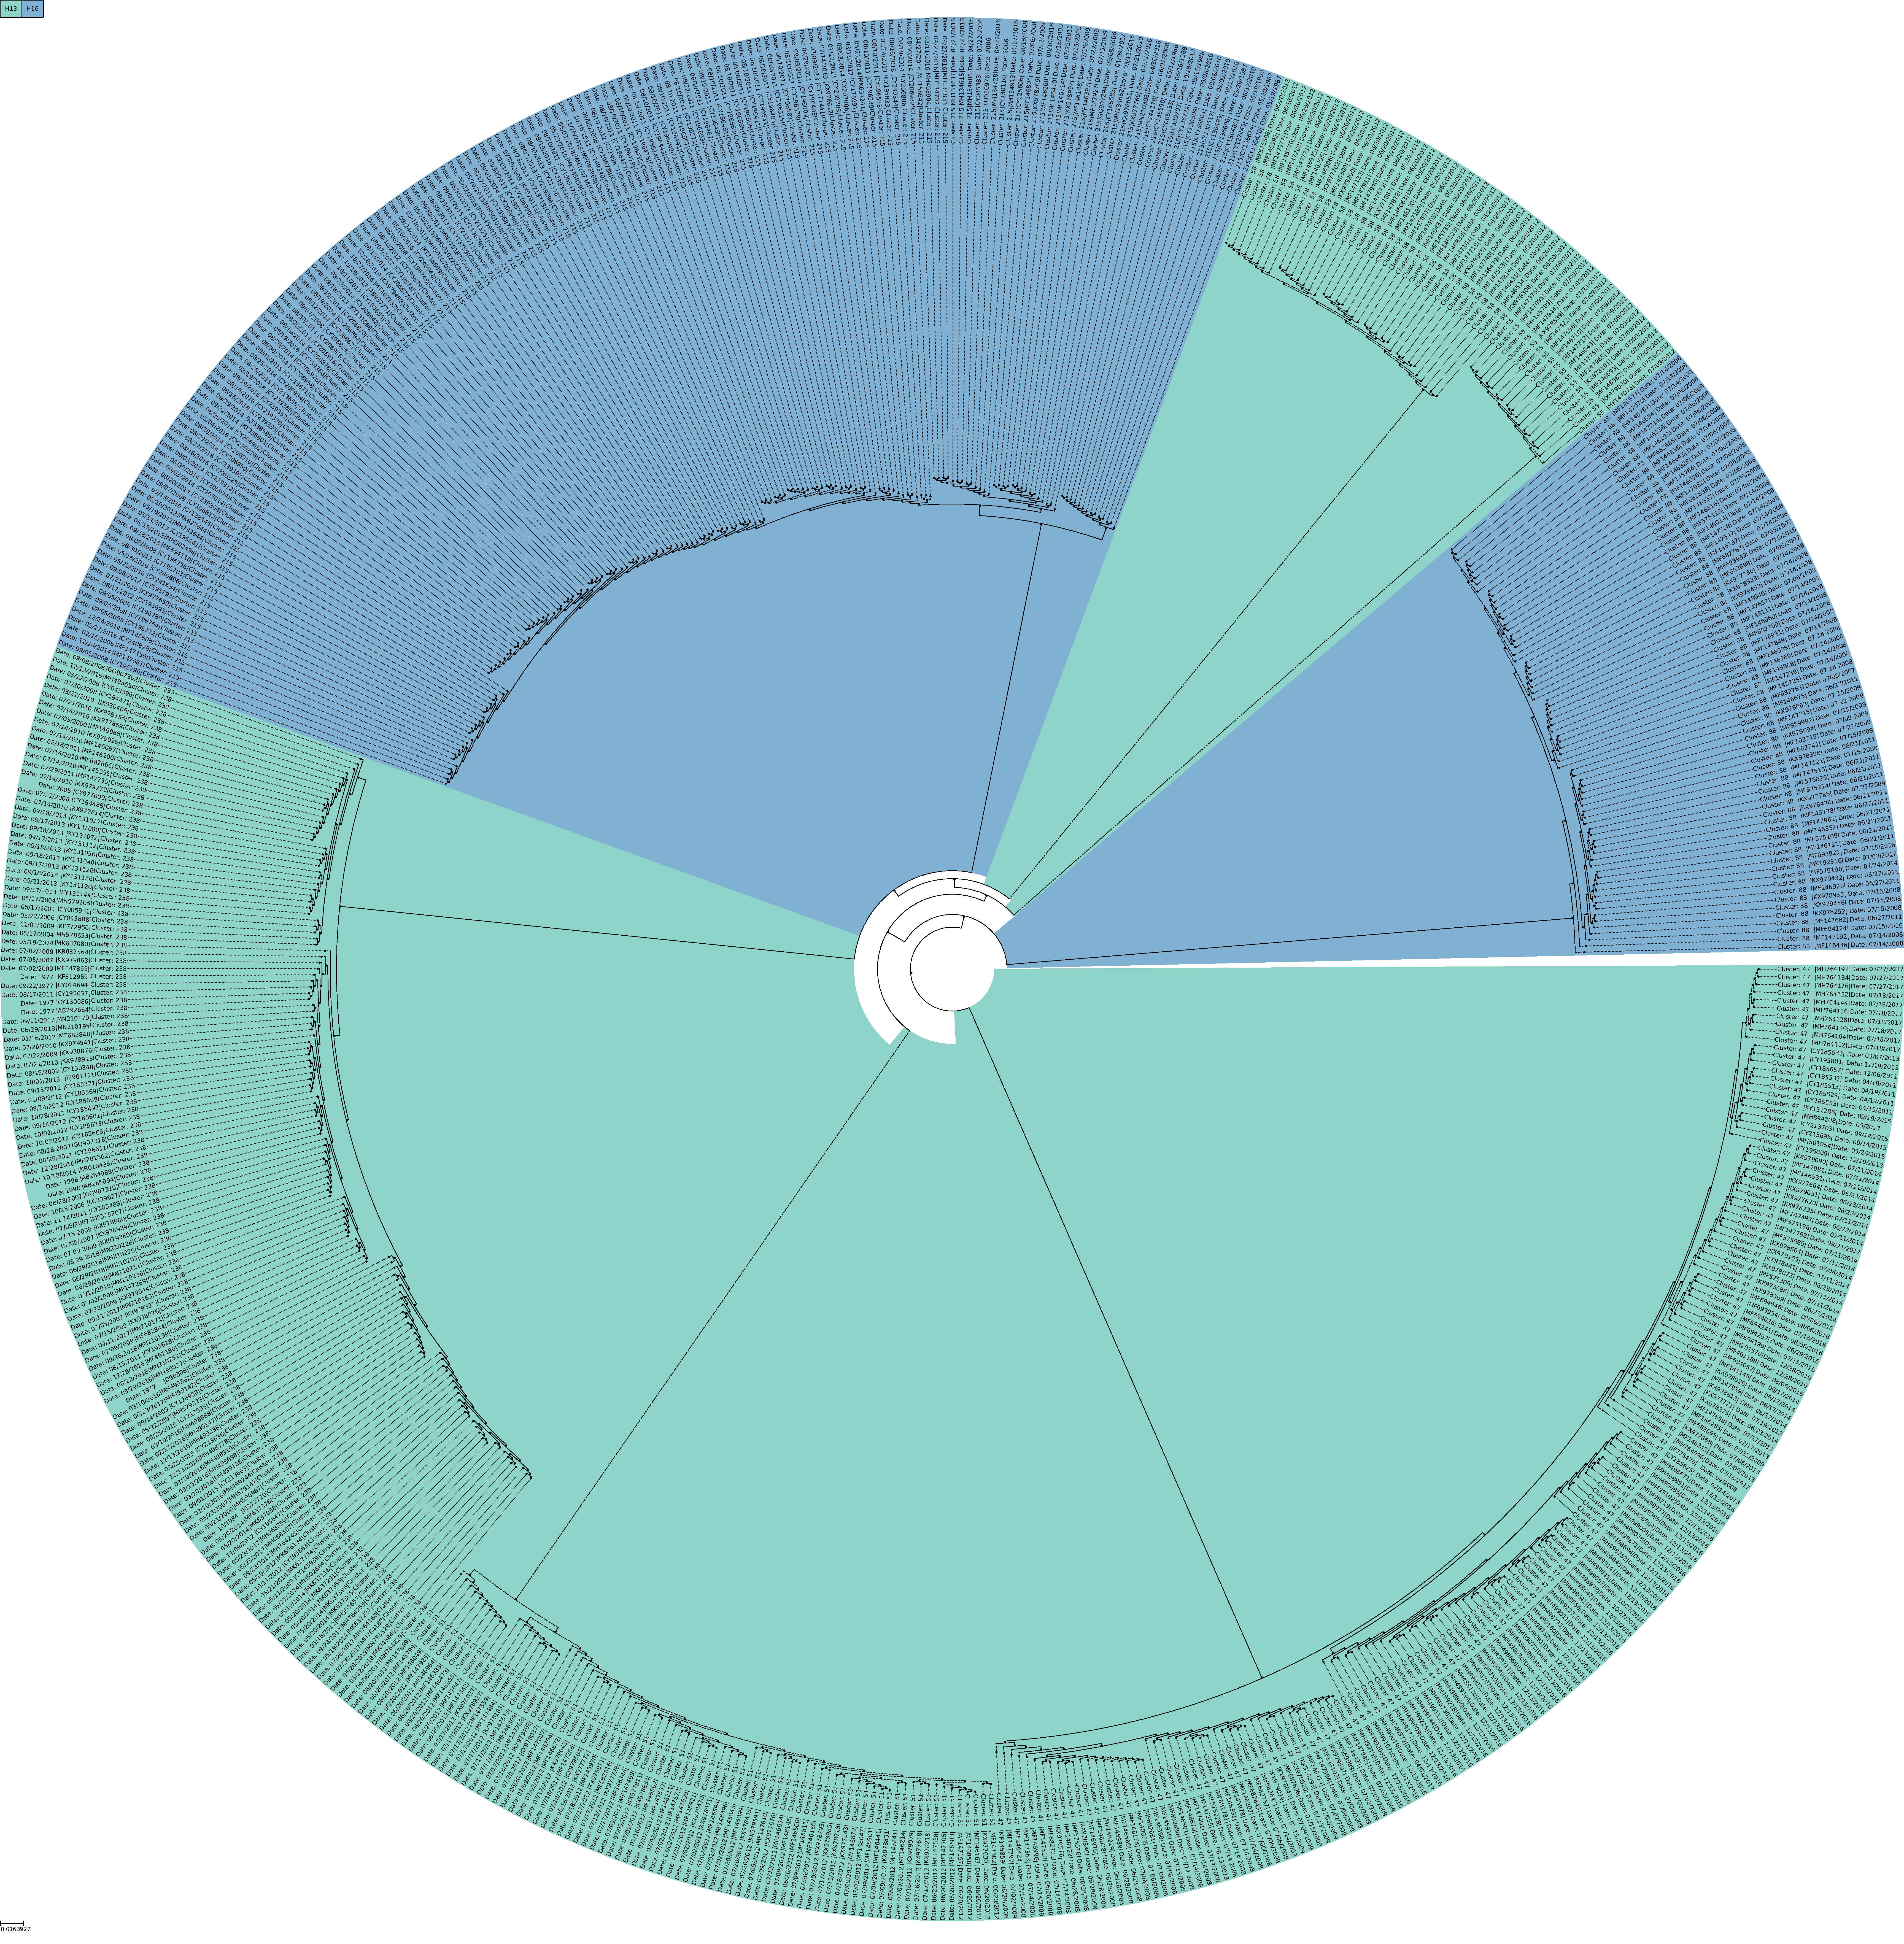
\includegraphics[width=\dimexpr\textwidth-2\fboxsep-2\fboxrule,fbox]{UMAP/Clustertree_Segment_4_H_Knee_Zoom.pdf}
%     \caption[H13/H16 Simple Clustering Example with \Acrshort{UMAP}]{\textbf{H13/H16 Simple Clustering Example with \Acrshort{UMAP}.} .}
%     \label{fig:UMAP_Clusteree_Knee_Zoom}
% \end{figure}

% \begin{figure}[!hbt]
%     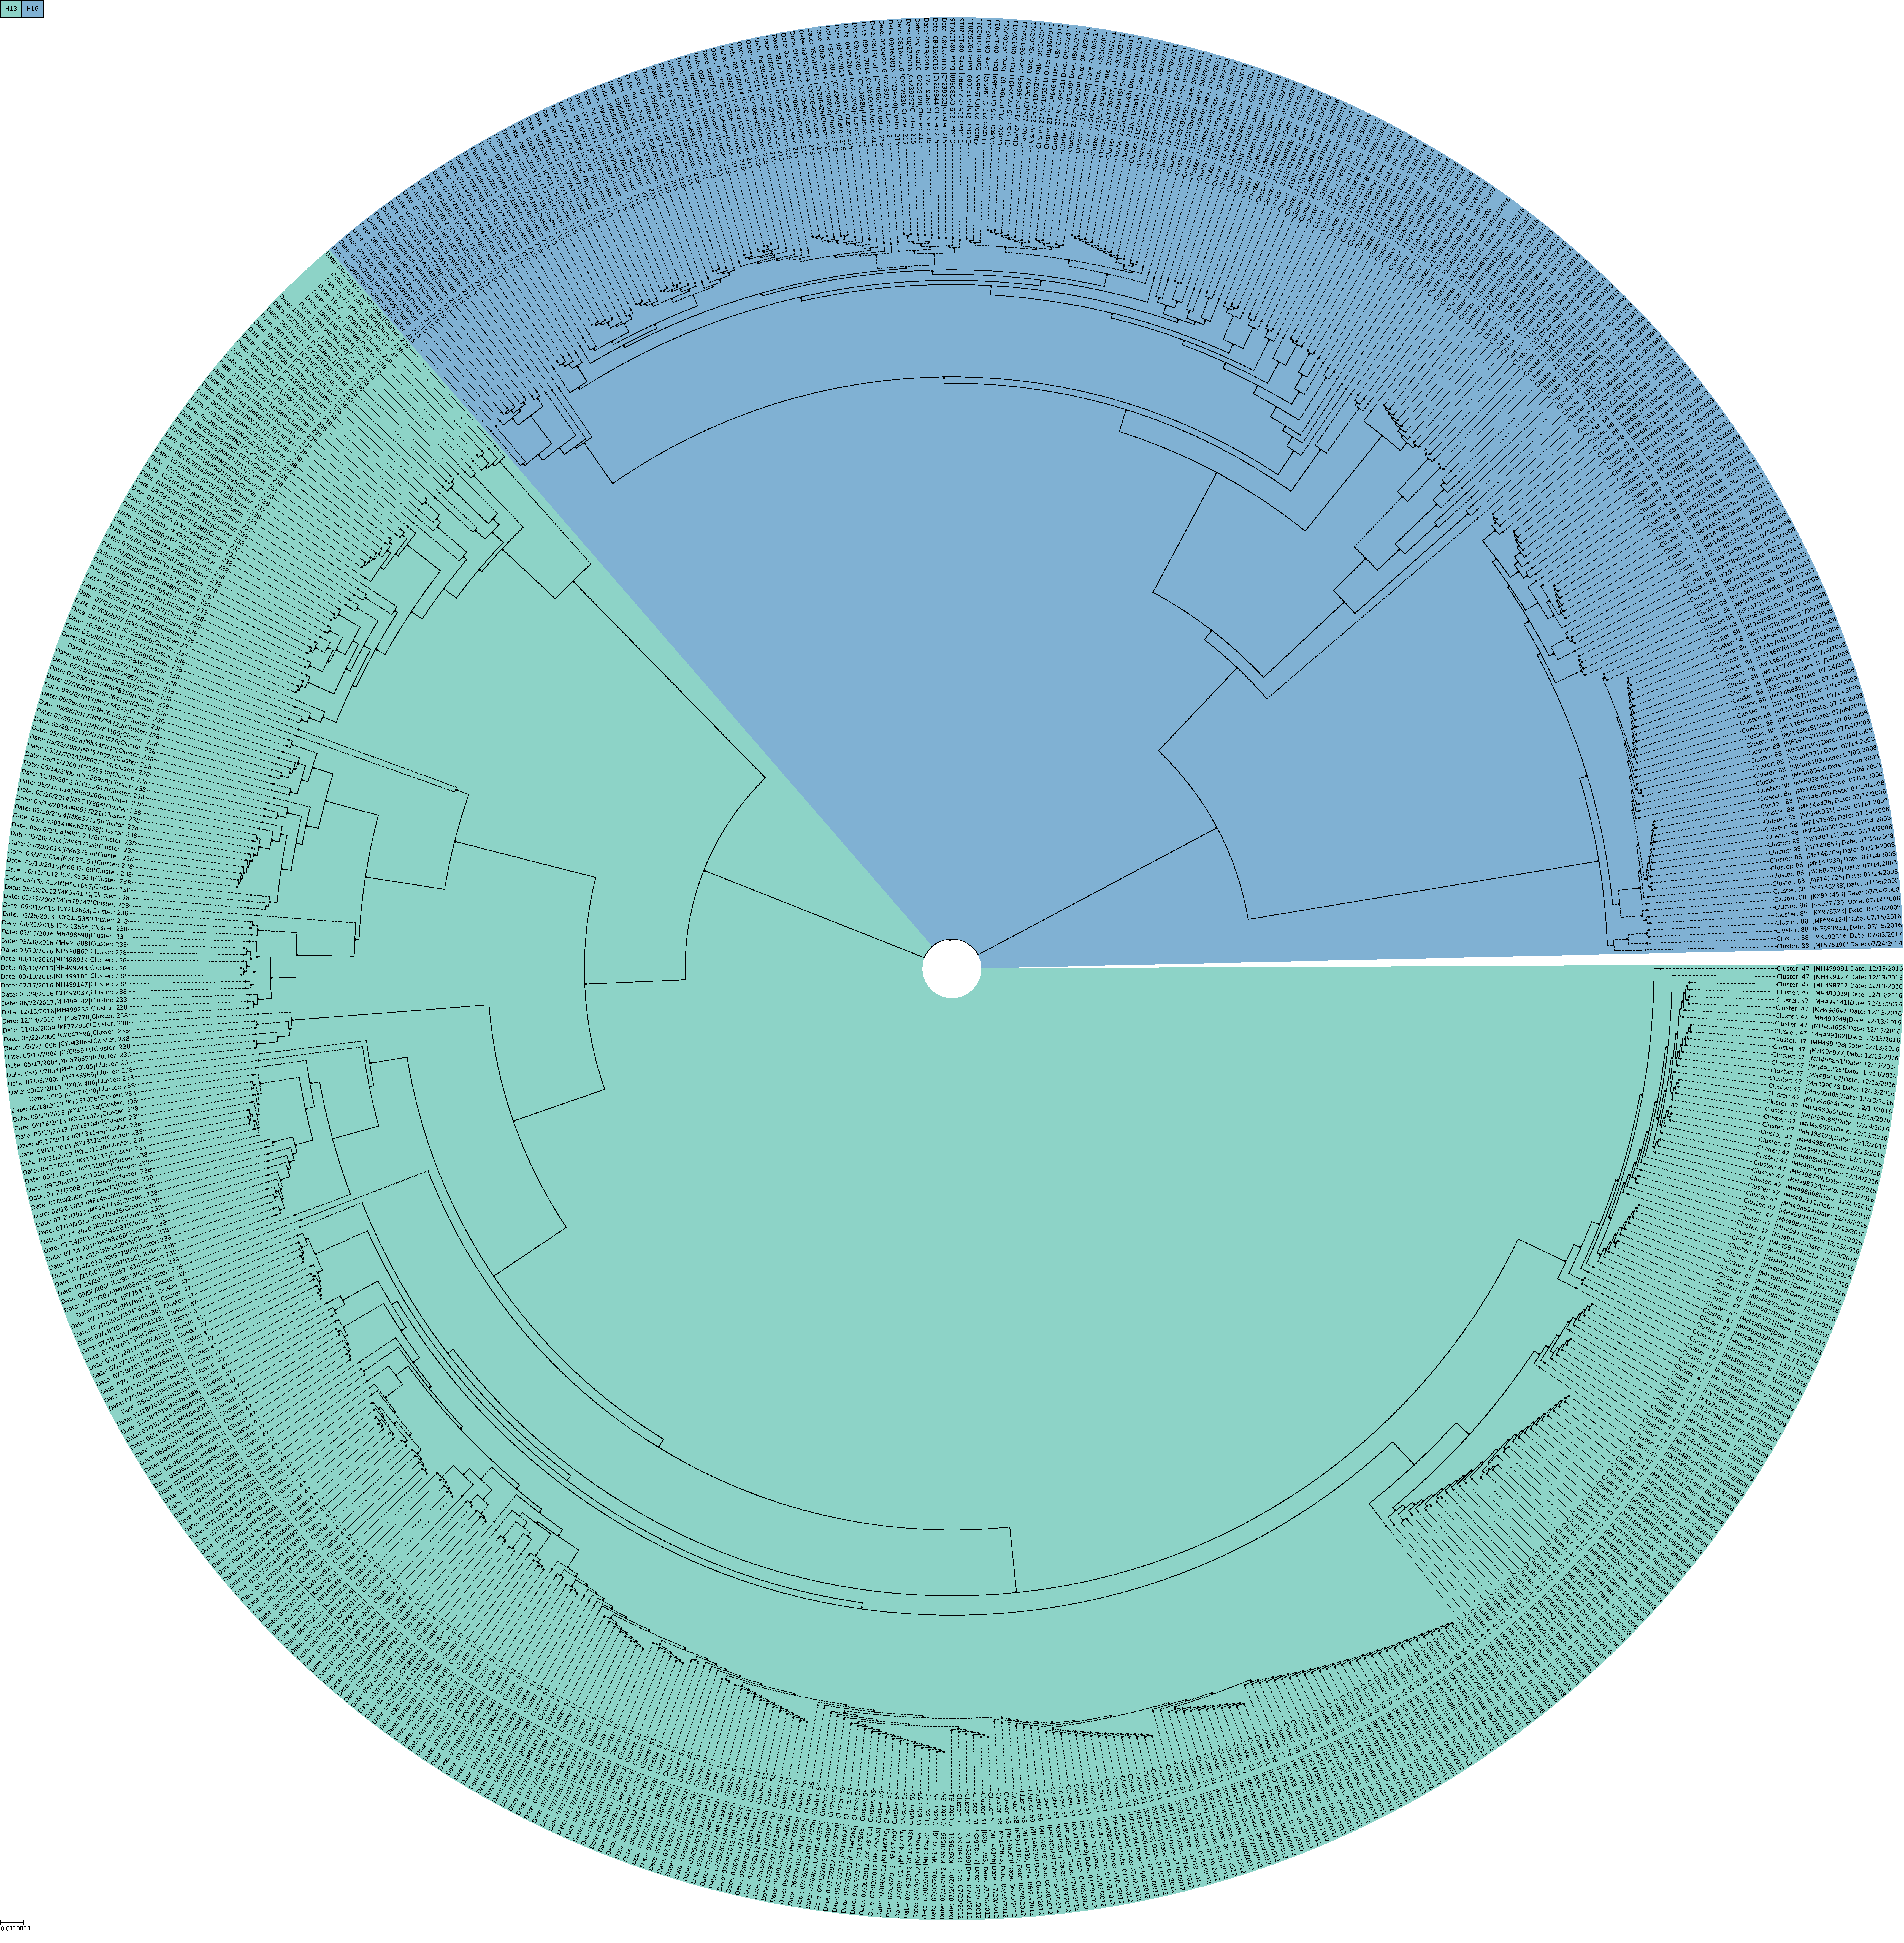
\includegraphics[width=\dimexpr\textwidth-2\fboxsep-2\fboxrule,fbox]{UMAP/Guidetree_Segment_4_H_Focus.pdf}
%     \caption[H13/H16 Simple Clustering Example with \Acrshort{MSA}]{\textbf{H13/H16 Simple Clustering Example with \Acrshort{MSA}.} .}
%     \label{fig:Guidetree_Focus}
% \end{figure}

\begin{figure}[!hbt]
    \centering
    \begin{tikzpicture}
        \node[anchor=south west,inner sep=0] (image) at (0,0) {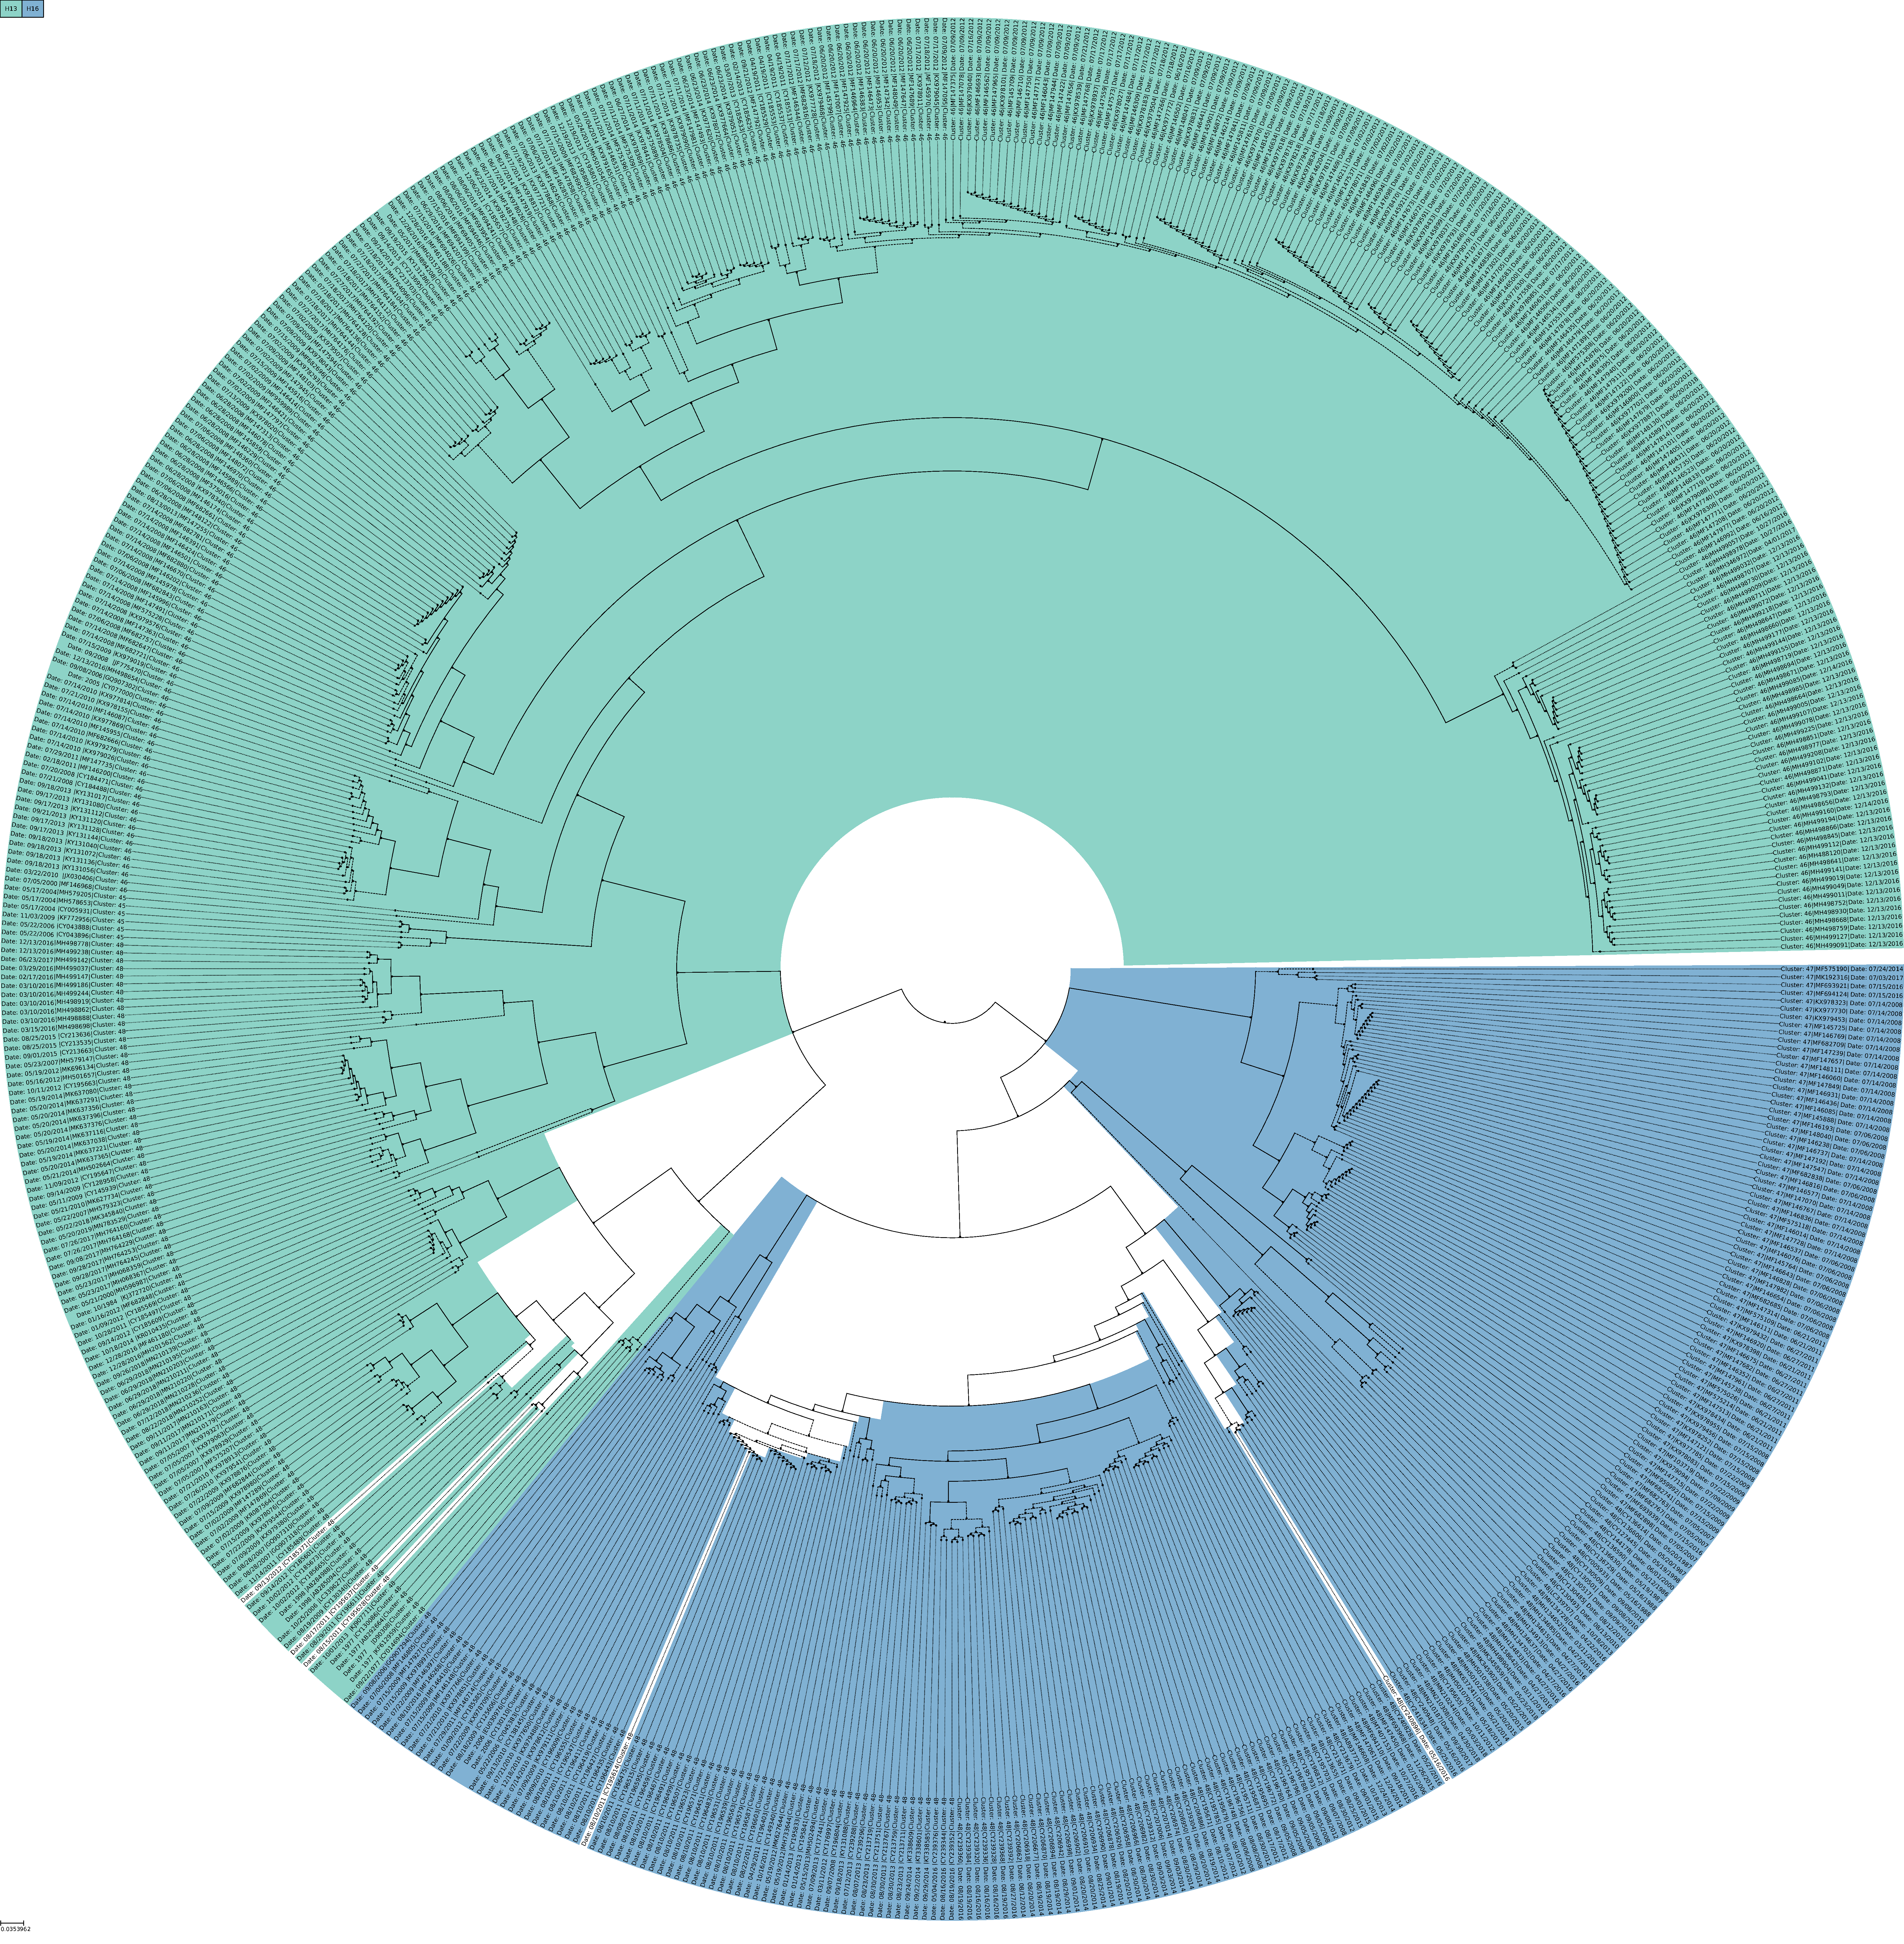
\includegraphics[width=\textwidth]{PCA/Precalculated_Segment_4_H_Cosine.pdf}};
        \begin{scope}[x={(image.south east)},y={(image.north west)}]
            %\draw[help lines,xstep=.1,ystep=.1] (0,0) grid (1,1);
            \draw[draw = none, fill = white] (0,1) rectangle (0.1,0.9);
            \draw[draw = none, fill = white] (0,0) rectangle (0.1,0.1);
            \draw[draw = black, thick, fill = black, fill opacity=0.2] (0.754,0.750) rectangle (0.999,0.505);
            \node at (0.754, 0.505) [fill=Red!80,thick,shape=circle,draw=black,inner sep=2pt] {\textbf{\textsf{B}}};
            \draw[draw = black, thick, fill = black, fill opacity=0.2] (0.344, 0.603) rectangle (0.589,0.358);
            \node at (0.344, 0.358) [fill=Red!80,thick,shape=circle,draw=black,inner sep=2pt] {\textbf{\textsf{A}}};
        \end{scope}
    \end{tikzpicture}
    \caption[H13/H16 Precalculated \Acrshort{UPGMA} Tree (cosine)]{\textbf{H13/H16 Precalculated \Acrshort{UPGMA} Tree (cosine).} .}
    \label{fig:Precalculated_Cosine}
\end{figure}

By building a \gls{UPGMA} tree on the non reduced segment 4 k-mer frequency vectors of the H13 and H16 subtypes the unbiased relation of sequences from these subtypes can be analyzed (\autoref{sec:MAFFT}). Also the fundamental use of k-mer frequencies can be validated or rejected. 
\begin{figure}[!hbt]
    \centering
    %\begin{adjustbox}{minipage=\dimexpr\textwidth-2\fboxsep-2\fboxrule,fbox}
    \begin{subfigure}[t]{0.475\textwidth}
        \caption{Subdivisions in the Subtypes}
        \label{subfig:root} 
        
        \begin{tikzpicture}
            \node[anchor=south west,inner sep=0] (image) at (0,0) {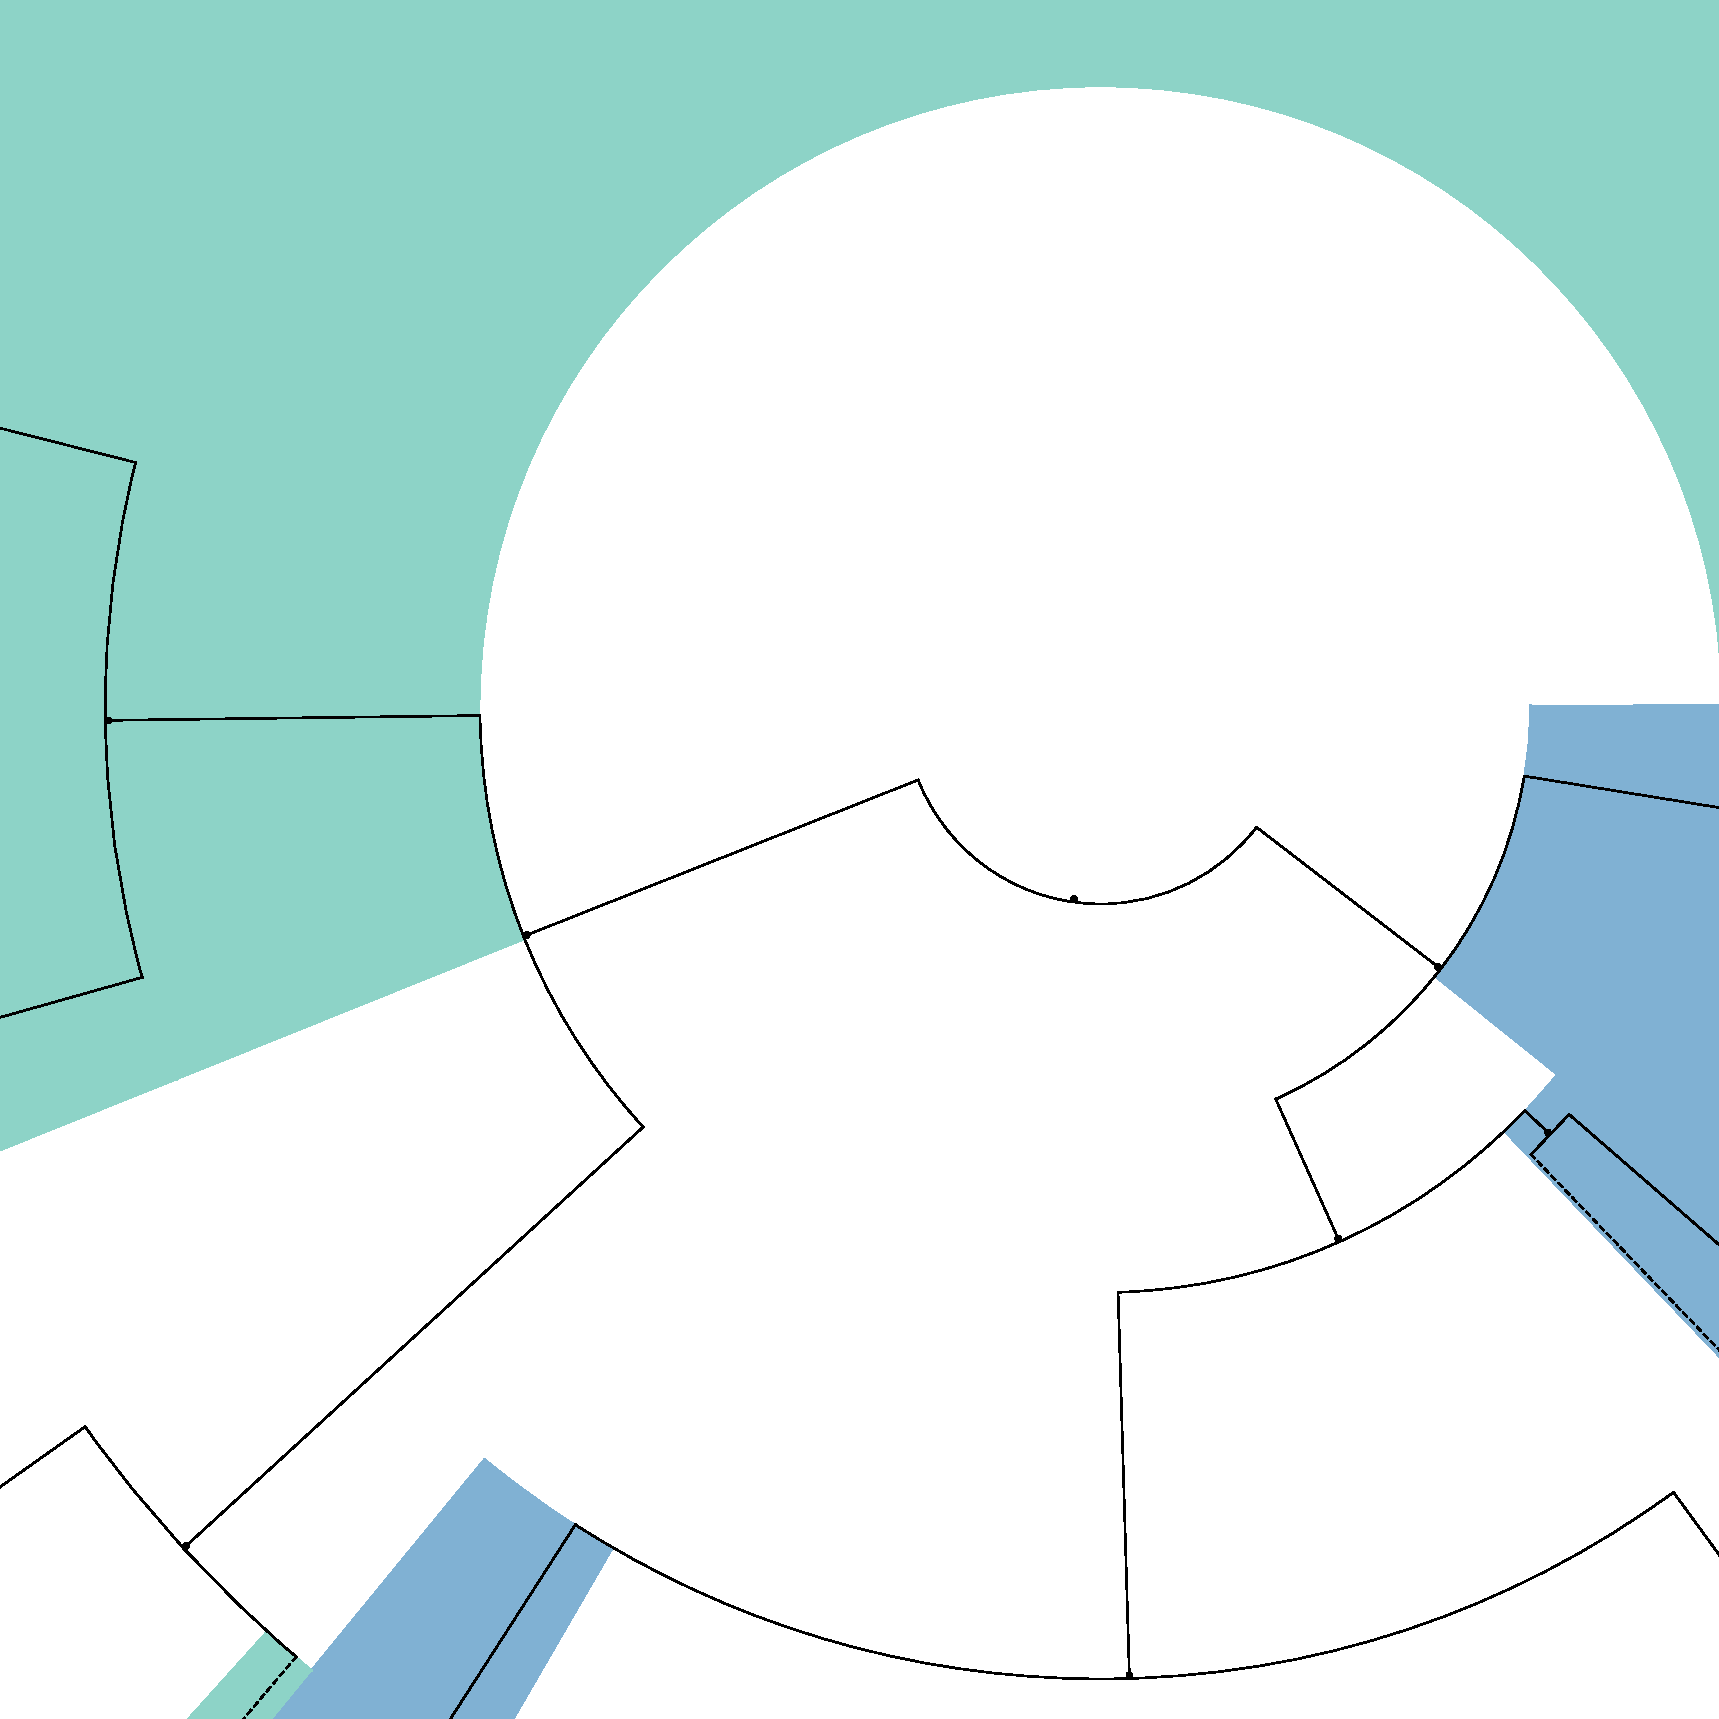
\includegraphics[width=\textwidth]{Graphics/root.pdf}};
            \begin{scope}[x={(image.south east)},y={(image.north west)}]
                %\draw[help lines,xstep=.1,ystep=.1] (0,0) grid (1,1);
                \node at (0.35,0.55) [arrowstyle=1.5cm, anchor=east, rotate=270] {\rotatebox{90}{\textbf{\textsf{A}}}};
                \node at (0.82,0.55) [arrowstyle=1.5cm, anchor=east, rotate=270] {\rotatebox{90}{\textbf{\textsf{B}}}};
            \end{scope}
        \end{tikzpicture}
    \end{subfigure}
    \hfill
    \begin{subfigure}[t]{0.475\textwidth}
        \caption{Difference in Analog sequences}
        \label{subfig:identical}
        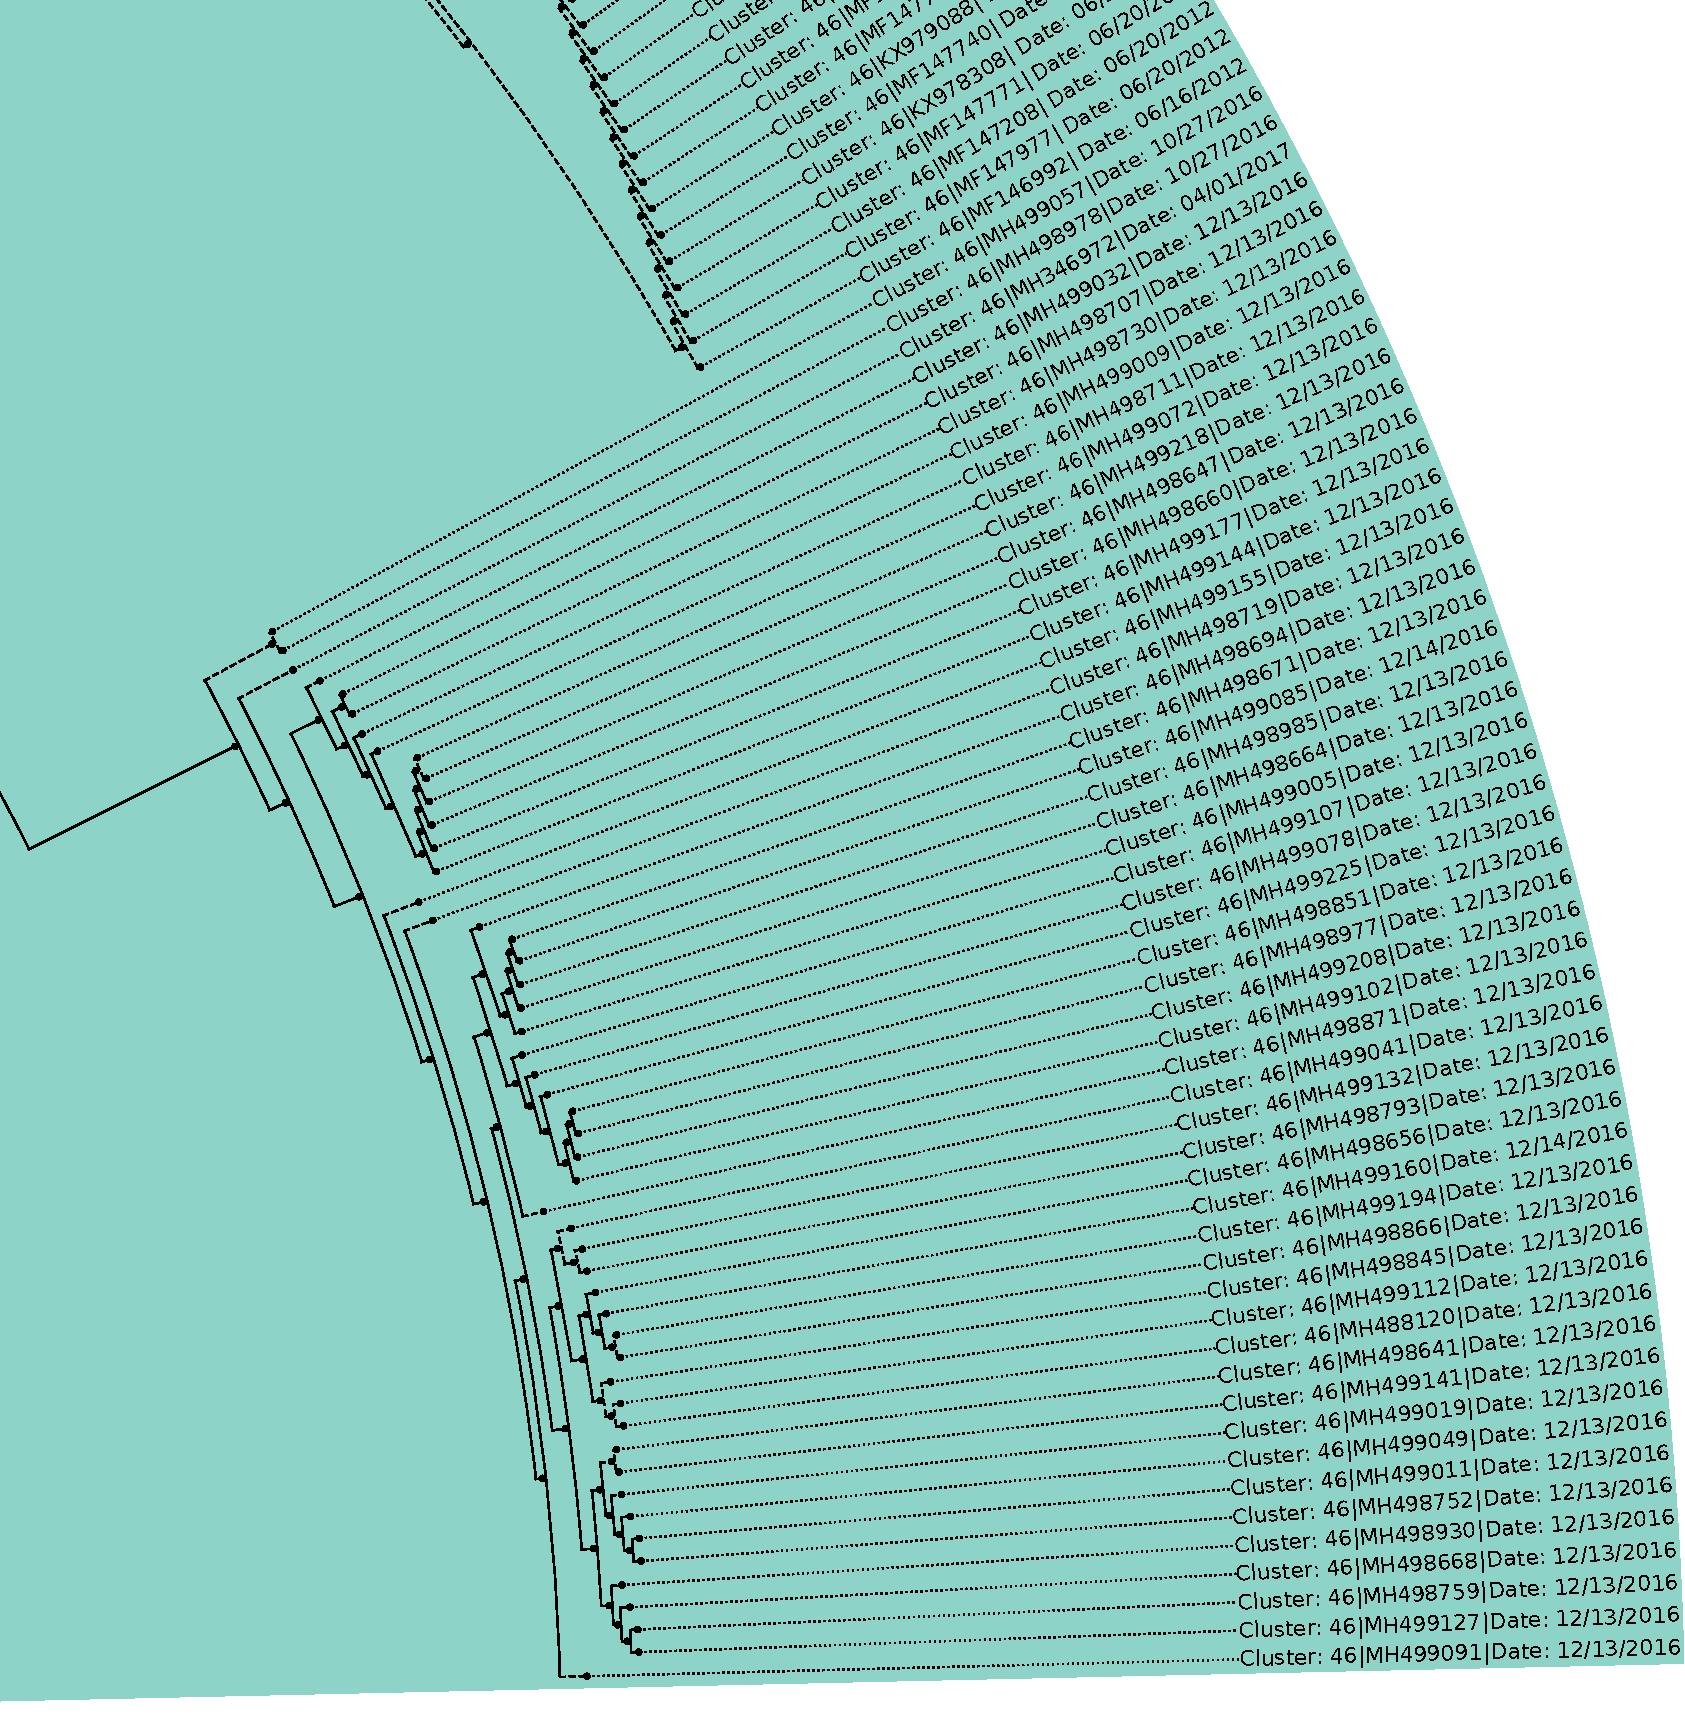
\includegraphics[width=\textwidth]{Graphics/identical.pdf}
    \end{subfigure}
    \caption[Focus in Precalculated \Acrshort{UPGMA} Tree]{Focus in Precalculated \Acrshort{UPGMA} Tree}
    \label{fig:focus}
\end{figure}

While both subtypes in \autoref{fig:Precalculated_Cosine} are completely seperated directly after the trees root, there are subdivisions for both subtypes directly after the seperation at the root. 

%frage is hier welche Methode die bessere representation ausstrahlt, sprich UMAP vgl. precalc ja/nein? dann PCA vgl precalc passt? ja/nein?